The proposed solution is to have 4 simple scale units. These units will simply recieve the analogue signal from a loadcell, convert it into an integer in digital form and then send that to a central unit via a wireless communication module. The central unit will recieve messages containing the weight from each of the 4 different scale units. It will then need to provide this information to a user in a standardised way in order to make it accessible from a generic device as required (see sec\ref{section:NFR}. See fig \ref{fig:Block Diagram} for a block diagram of the prosed design.

%This approach of using the central unit to host the information on a network means that any device capable of %connecting to the network and displaying a webpage, will easily be able to manipulat the system and retreive %information. This fits the requirement of being accessible from a generic handheld device such as a phone or %tablet found in ref{section:NFR}.
\subsection{Scale Units}
\label{scale}
These units are where the majority of the work is done, they are essentially load cell control units. This means that they are the responsible for interfacing to the base analogue output of the load cell, configuring it into a manageable form and then transmitting it to the central unit. This will require several components: cheifly some form of microcontroller with an anologue to digital converter, a wireless communication device, a circuit that travels through a load cell into a wheatstone bridge and then into an instrumentation amplifier in order to increase accuracy. 
\subsection{Central Unit}
\label{central}
This is the central hub of the system; where all the information is brought together, analysed and provideded to the user of the system. This component will need a microcontroller and a wireless communication device capable of communicating with all 4 of the scale units. It will then need to provide this information to a user in a standardised way in order to make it accessible from a generic device as required"

\begin{figure}
\begin{center}
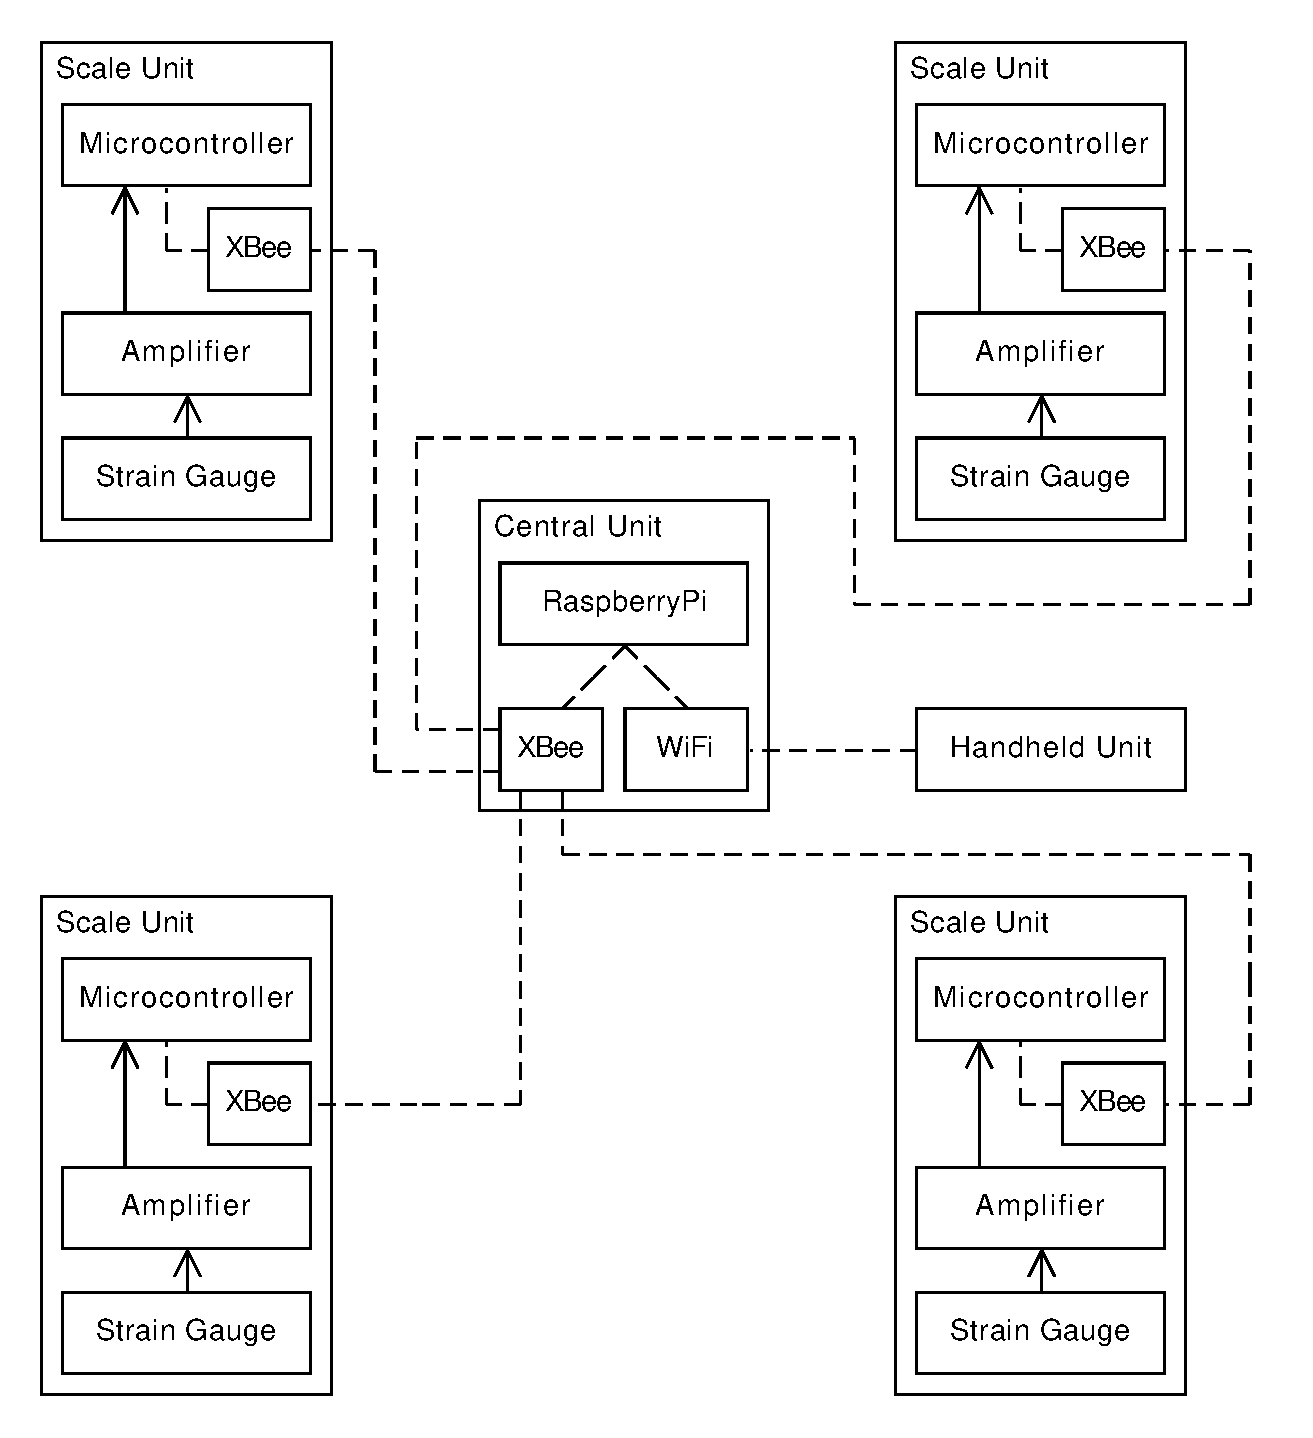
\includegraphics[width=12cm]{figures/block_diagram}
\end{center}
\caption{Block Diagram}
\label{fig:Block Diagram}
\end{figure}
